%!TEX root = thesis.tex

\documentclass[12pt]{article}
\usepackage[utf8]{inputenc}
\usepackage[spanish,es-ES]{babel}

% Margenes
\usepackage{geometry}
\geometry{
  letterpaper,
  top=4cm,
  bottom=3cm,
  left=4cm,
  right=3cm
}

% Fuente
\usepackage{times}
\usepackage{csquotes}

\renewcommand{\baselinestretch}{1.5}

\usepackage{graphicx}
\usepackage{hyperref}
\usepackage{float}
\usepackage{parskip}
\usepackage[spanish]{cleveref}

\usepackage[caption = true]{subfig}

\usepackage[backend=biber,style=apa,language=spanish]{biblatex}
\bibliography{biblio}

\begin{document}

\title{Análisis Descriptivo y Predictivo Basado en Datos del Tráfico Vehicular en Antofagasta: Un Enfoque a partir de Reportes de Conductores}
\author{Richard Peña Bonifaz}
\date{\today}
\maketitle

\section*{Dedicatoria}
A nadie.
\section*{Reconocimientos}
A mí.
% \tableofcontents
% \newpage

\section*{Resumen}

El presente proyecto tiene como propósito desarrollar una herramienta efectiva para analizar y predecir, con alta confiabilidad, el comportamiento del tráfico vehicular en la ciudad de Antofagasta mediante el uso de datos provenientes de la plataforma Waze Cities. Waze, a través de su comunidad de usuarios, ofrece información en tiempo real que permite obtener una visión detallada de los eventos de tráfico que ocurren en la ciudad. Esta investigación genera información relevante para la gestión del tráfico, facilitando la toma de decisiones por parte de las autoridades locales con el fin de mejorar la seguridad vial y optimizar la eficiencia del flujo vehicular. A través del análisis y explotación de estos datos, se identifican patrones y tendencias que, integrados en la planificación urbana, contribuirán a optimizar rutas críticas, reducir la congestión y minimizar la probabilidad de accidentes.

En este estudio se emplearán técnicas de análisis de datos y métodos geoespaciales mediante el uso de la librería GeoPandas en Python, además de la aplicación de series temporales para proporcionar visualizaciones claras y comprensibles dirigidas al usuario final. Adicionalmente, se implementarán técnicas de aprendizaje automático para realizar predicciones de tráfico, anticipándose a eventos y contribuyendo al desarrollo urbano eficiente y seguro \parencite{barcelo2005}.

\section{Introducción}
\subsection{Descripción del problema}

Antofagasta, una ciudad con más de 106,000 vehículos en circulación \parencite{comision2023}, enfrenta desafíos significativos en la gestión de su tráfico vehicular. Durante el año 2023, se registraron 1,715 accidentes, los cuales resultaron en 31 fallecidos y 102 heridos graves \parencite{comision2023}. La infraestructura vial limitada, sumada a la alta concentración de vehículos en un número reducido de arterias principales, agravó la congestión y elevó el riesgo de accidentes. A pesar de la existencia de estos problemas, no se cuenta con sistemas de monitoreo en tiempo real que permitan gestionar el tráfico de manera proactiva. Por ello, se aprovecharán fuentes de datos alternativas, como Waze, para recolectar información valiosa que facilite la toma de decisiones en materia de tráfico \parencite{chen2015}.

\subsection{Objetivo general}

Realizar un análisis exhaustivo del comportamiento del tráfico en la ciudad de Antofagasta basado en los eventos reportados por los conductores en la plataforma Waze. El objetivo final es generar información relevante que contribuya a la gestión eficiente del tráfico, mejorando la seguridad vial y optimizando el flujo vehicular.

\subsection{Objetivos específicos}

\begin{itemize}
    \item Obtener datos suficientes y representativos sobre los eventos de tráfico en Antofagasta mediante la API de Waze Cities.
    \item Realizar un análisis descriptivo de los datos recolectados para identificar patrones y tendencias relevantes en el comportamiento del tráfico.
    \item Identificar los factores clave que influyen en la seguridad vial y la eficiencia del tráfico en la ciudad.
    \item Presentar información visualmente comprensible y útil para las autoridades de gestión vial, facilitando la implementación de políticas y acciones basadas en datos \parencite{auld2009}.
    \item Utilizar los datos disponibles para desarrollar modelos predictivos de tráfico que permitan anticipar eventos y tomar decisiones proactivas en la gestión vial.
\end{itemize}

\section{Marco teórico}

El tráfico vehicular en entornos urbanos presenta un comportamiento complejo e impredecible, lo que dificulta su gestión eficiente. No obstante, el avance de las tecnologías móviles y la popularidad de aplicaciones como Waze permiten disponer de datos en tiempo real generados por los propios usuarios. Este proyecto se apoya en técnicas de análisis de datos y aprendizaje de máquinas (Machine Learning) para convertir esta información en herramientas útiles para la gestión vial. La utilización de datos geoespaciales, junto con la automatización de los procesos de recolección, análisis y visualización, constituye una solución costo-efectiva para mejorar la planificación del tráfico \parencite{barcelo2005}.

\subsection{Metodología}

Una de las principales limitaciones en el análisis de fenómenos es la ausencia de datos suficientes y debidamente estructurados. Por ello, se diseñó una estrategia de recolección de datos que garantizara conclusiones con un nivel adecuado de certeza. La API de Waze Cities, que proporciona información en tiempo real sobre eventos activos, fue la fuente principal de datos. Para lograr un volumen de datos representativo, se implementó un servidor encargado de recopilar y almacenar esta información de manera continua.

Se realizó un análisis geoespacial con el objetivo de identificar puntos críticos, como vías principales, calles secundarias y zonas de alto tráfico. Este análisis se llevó a cabo utilizando GeoPandas, una herramienta de Python especializada en operaciones geoespaciales. Además, se analizaron series temporales para detectar patrones y tendencias del tráfico, identificando estacionalidades en el comportamiento. Los resultados se presentaron mediante técnicas de visualización que permitieron interpretar las tendencias y puntos de interés de manera efectiva.

El pipeline de datos incluyó una base de datos relacional para almacenar los datos, un flujo ETL (Extract, Transform, Load) para procesarlos y un servidor web para visualizarlos. Se utilizó PostgreSQL como base de datos, APScheduler para la programación de tareas y Dash como herramienta de visualización. Este enfoque permitió automatizar el flujo de datos y garantizar la actualización constante de la información.

Adicionalmente, se entrenó un modelo de clasificación para determinar la probabilidad de ocurrencia de accidentes en diferentes puntos de la ciudad. El modelo seleccionado fue XGBoost, el cual fue seleccionado utilizando técnicas de validación cruzada y optimización de hiperparámetros. Los resultados obtenidos permitieron identificar las variables más influyentes en la ocurrencia de accidentes, así como la probabilidad de ocurrencia en diferentes condiciones de tráfico. Para la selección de variables se utilizó GridSearchCV, una técnica de búsqueda de hiperparámetros que permite encontrar la mejor combinación de variables para el modelo, se compararon modelos de regresión logística, árboles de decisión y XGBoost, siendo este último el que presentó el mejor desempeño en términos de precisión y sensibilidad.

Para la gestión del modelo, en cuanto a su implementación, mantenimiento y actualización, se programó con APSCheduler, una librería de tareas asíncronas en Python, que permite gestionar el ciclo de vida de los modelos de aprendizaje automático, desde su entrenamiento hasta su despliegue en producción y versionado.

En la parte del servidor, se desarrolló en Rust, un lenguaje de programación enfocado en la eficiencia en el uso de memoria y seguridad en el uso de la misma. Se utilizó la herramienta Memcached para generar un caché de los datos y de esta forma poder servirlos de manera más eficiente y rápida, debido al volumen de dato, se priorizó la unicidad de los datos, evitando generar copias, para no aumentar el uso de memoria.

Para el procesado de los datos en el cliente (Dash), se generan multiples workers que permiten servir la aplicación de forma eficiente, y se utiliza solo una instancia en memoria de los datos, compartidos por todos los datos, y para mantener la integridad de los datos, se implementó un Mutex para controlar el acceso de lectura a los mismos desde las tareas asíncronas.

La perspectiva general del flujo de datos se muestra en la \autoref{fig:fuente} y el flujo desde la API de Waze hasta el dashboard se puede observar en la \autoref{fig:wf_dash}

\begin{figure}[h]
    \centering
    \includegraphics[width=0.8\textwidth]{diagrams/fuente_datos.png}
    \caption{Pipeline general de datos}
    \label{fig:fuente}
\end{figure}

\begin{figure}[h]
    \centering
    \includegraphics[width=0.8\textwidth]{diagrams/wf_dash.png}
    \caption{Flujo de información en dashboard}
    \label{fig:wf_dash}
\end{figure}

\section{Desarrollo}

Para obtener los datos necesarios para el análisis, fue necesario generar un mecanismo para recolectar y almacenar la información de Waze Cities. Se implementó un servidor que se encarga de realizar peticiones a la API de Waze, recolectar los eventos de tráfico y almacenarlos en una base de datos PostgreSQL. Este servidor se ejecutaba de manera continua, actualizando la información cada 2 minutos. La estructura de la base de datos se muestra en la \autoref{fig:db_diagram}.

\begin{figure}[H]
    \centering
    \includegraphics[width=0.8\textwidth]{images/db_diagram.png}
    \caption{Diagrama de la base de datos}
    \label{fig:db_diagram}
\end{figure}

Existen dos estructuras principales, las alertas (alerts) y las congestiones (jams), el primero registra todos los eventos reportados por usuarios, tales como peligros, accidentes, congestión o rutas cerradas. En el caso de los eventos de congestión, son datos generados automáticamente por Waze, los cuales usando la geolocalización, estiman congestiones en diferentes puntos de la ciudad. Para este proyecto, se utilizó la información de las alertas. Sin embargo, se almacenaron los datos de congestión, para un posterior análisis, que está fuera del alcance de este estudio. Esta estructura se definió con base en los datos relevantes y completos que proporciona la API, los tipos de datos disponibles pueden ser consultados en la documentación de Waze \parencite{waze2024}.

Desde octubre de 2024 hasta Abril de 2025, se han acumulado 40429 alertas, las cuales se analizarán a lo largo de esde estudio.


\subsection{Eventos en el espacio y tiempo}

En la \autoref{fig:dist_events} se muestran como los difentes tipos de eventos se distribuyen a lo largo de la ciudad, teniendo concentraciones las avenidas principales y en el caso de accidentes, en los cruces entre ellas.


\begin{figure}[H]
    \centering
    \subfloat[Accidentes]{
        \includegraphics[width=0.33\textwidth]{images/dist_accidents.png}
    }
    \subfloat[Congestión]{
        \includegraphics[width=0.33\textwidth]{images/dist_jams.png}
    }
    \subfloat[Peligros]{
        \includegraphics[width=0.33\textwidth]{images/dist_hazards.png}
    }
    \caption{Distribución de eventos en Antofagasta}
    \label{fig:dist_events}
\end{figure}

Para realizar el análisis de tiempo, se agruparán los eventos por hora de ocurrencia en el día, tomando el promedio de eventos ocurridos al día. En la \autoref{fig:time_events}, los eventos se concentran en los horarios punta, tanto para accidentes como para congestión, para el caso de peligro, se observa una distribución más uniforme durante el día.

\begin{figure}[H]
    \centering
    \subfloat[Accidentes]{
        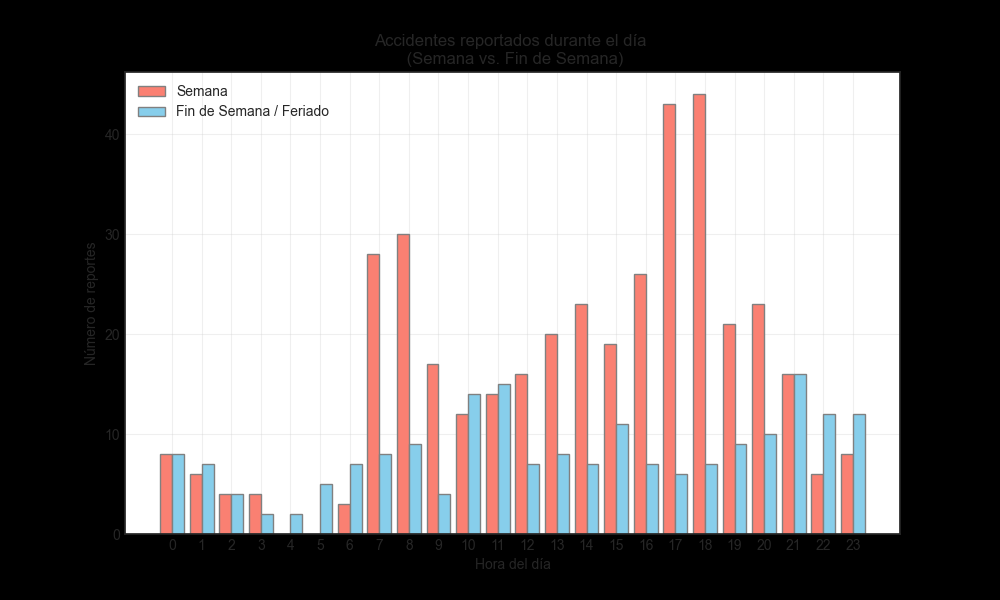
\includegraphics[width=0.6\textwidth]{images/ACCIDENT_per_hour.png}
    }
    \newline
    \subfloat[Congestión]{
        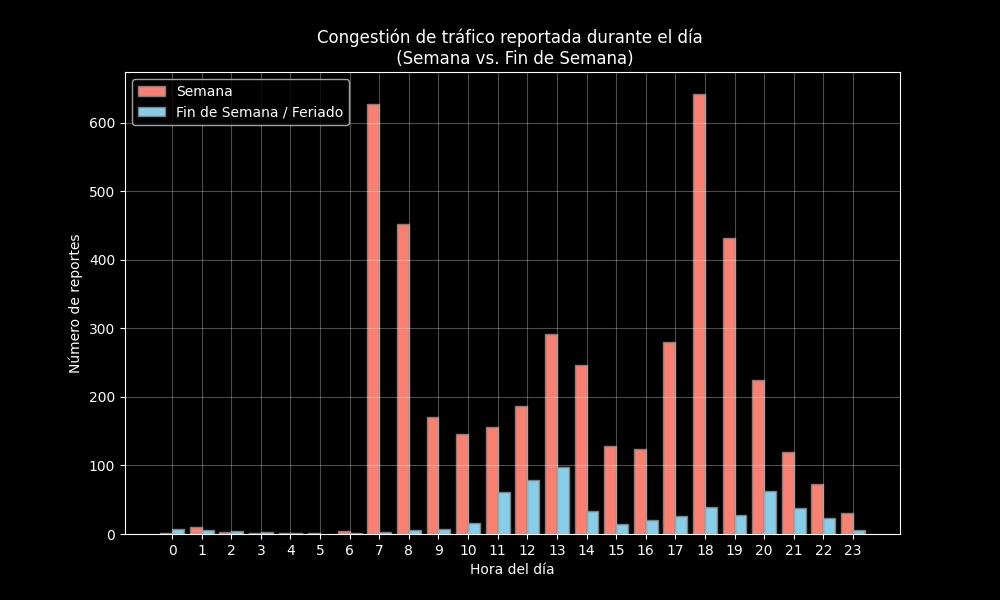
\includegraphics[width=0.6\textwidth]{images/JAM_per_hour.png}
    }
    \newline
    \subfloat[Peligros]{
        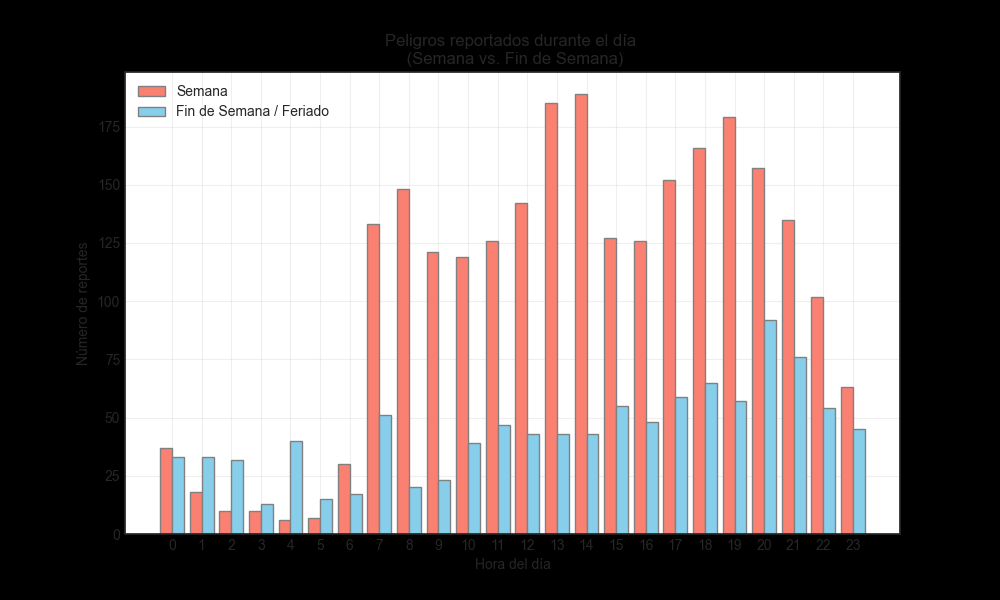
\includegraphics[width=0.6\textwidth]{images/HAZARD_per_hour.png}
    }
    \newline
    \caption{Eventos según hora del día en Antofagasta}
    \label{fig:time_events}
\end{figure}

% Prueba hipótesis relación accidents-jams


\begin{figure}[H]
    \centering
    \subfloat[Día de semana]{
        \includegraphics[width=0.9\textwidth]{images/corr_lin_ds.png}
    }
    \newline
    \subfloat[Fin de semana]{
        \includegraphics[width=0.9\textwidth]{images/corr_lin_fs.png}
    }
    \newline
    \caption{Correlación lineal entre accidentes y congestión}
    \label{fig:corr_lineal}
\end{figure}


\begin{figure}[H]
    \centering
    \subfloat[Día de semana]{
        \includegraphics[width=0.9\textwidth]{images/corr_exp_ds.png}
    }
    \newline
    \subfloat[Fin de semana]{
        \includegraphics[width=0.9\textwidth]{images/corr_exp_fs.png}
    }
    \newline
    \caption{Correlación exponencial inversa entre accidentes y congestión}
    \label{fig:corr_exp}
\end{figure}

% Cálculo de la frecuencia por zona
% Filtro por zona
%    Algóritmo cKDTree

\subsection{Frecuencia por zona}
Para representar conjuntos estáticos de puntos espaciales, se utiliza la estructura cKd-tree, una variante compacta del Kd-tree que codifica distancias relativas mediante spiral codes y las almacena usando Directly Addressable Codes (DACs), optimizando el uso de memoria sin sacrificar eficiencia en consultas espaciales \parencite{gutierrez2023ckdtree}. A cada zona la llamaremos grupo o segmento.

% Ruta más segura

% Machine learning (XGBoost)

% Aplicación implementacióñ (dashboard online y ML)

% \section{Resultados}

% Observaciones y resultados del estudio

% \section{Discusión}

% Preguntas y posibles soluciones

% \section{Conclusiones}

% Conclusión según los resultados

% \section{Recomendaciones}

% Propuesta de solución o nuevo estudio

\printbibliography

\end{document}

